\chapter{基础理论}
多目标跟踪技术在智能感知与视觉理解等领域具有重要应用价值,其核心难点在于复杂场景下的轨迹关联与身份保持。
为更好地理解本文后续提出的多目标跟踪与跨域自适应方法,本章对相关基础理论进行介绍。首先阐述图的基本概念及图神经网络的核心原理,
为基于图结构的轨迹关联方法提供理论支撑;随后介绍跨域视觉感知与自适应建模的基本思想,
分析恶劣视觉条件引起的域偏移问题;最后给出本文实验中使用的数据集与评价指标。
\section{图神经网络相关理论及方法}
图神经网络是一类能够直接作用于图结构数据的深度学习模型,在建模非结构化数据及复杂关系方面具有显著优势。
鉴于多目标跟踪中的轨迹关联问题天然具备图结构特性,引入图神经网络为刻画目标之间的关联关系提供了有效工具。
为系统介绍图神经网络的相关理论,本节首先从图的基本概念出发,阐述节点、边及其特征的表示方式,
并简要介绍图神经网络在不同层级任务中的应用。
随后,对图神经网络的谱域与空域方法进行分类说明,重点介绍基于消息传递机制的空域建模方法。
\subsection{图神经网络基本理论及应用}
\textbf{1. 图基本概念}

图(Graph)是一种用于描述对象及其交互关系的基本数据结构,广泛应用于具有复杂关系的非结构化数据。
假设一个图$G$包含$M$个节点和$N$条边,节点集合用$V=\{v_1,v_2,\cdots,v_M\}$表示,每个节点$v_i$可以表示成一个实体(如视频帧中的一个检测目标)。
边集合$E$用于描述节点之间的连接关系,定义为$E=\lbrace e_{ij} = (v_i,v_j) ~ |~ v_i,v_j\in V,\quad |E|=N \rbrace$,
其中$e_{ij}$表示从节点$v_i$指向节点$v_j$的一条边。
在无向图中,$e_{ij}$与$e_{ji}$表示同一条边;而在有向图中,$e_{ij}$与$e_{ji}$表示两条方向相反、相互独立的有向边。
综上,图$G$可形式化表示为$G=(V,E)$,由节点集合和边集合共同构成。

在实际计算中,图的连接关系通常采用邻接表(Adjacency List)等稀疏数据结构进行存储,以提升在大规模图上的计算与存储效率。
对于无向图,每一条边需要在相邻两个节点的邻接表中分别存储一次;而对于有向图,每条边仅需存储一次。
因此,在采用邻接表表示的情况下,无向图在存储开销上通常是对应有向图的两倍(假设边数量相同)。

除了结构信息外,图通常还具备丰富的特征信息。节点属性矩阵一般表示为$X_v\in \mathbb{R}^{M\times C_v}$,其中$C_v$是每个节点的特征数,可包含外观、运动、空间位置等属性;
边属性矩阵则表示为$X_e \in \mathbb{R}^{N\times C_e}$,其中$C_e$是每条边的特征数,用于刻画节点之间的关系属性,如相对位移、时序间隔、相似度度量或关系类型等。

图神经网络的目标是通过结合图结构信息和节点、边属性,学习到更高级的节点嵌入(节点$v_i$的嵌入表示为$h_i$)和边嵌入(边$e_{ij}$的嵌入表示为$z_{ij}$),
从而支撑各类图分析任务。

\autoref{tab:ch2_1}给出了本文图神经网络建模中涉及的主要概念及其对应符号。

\begin{table}[htbp]
    \caption{\label{tab:ch2_1}图神经网络建模中主要概念及其对应符号}
    \begin{tabularx}{\linewidth}{c|X<{\centering}}
        \hline
        \textbf{概念} & \textbf{符号} \\ \hline
        节点数量 & $M$ \\ \hline
        节点集合 & $V=\{v_1,v_2,\cdots,v_M\}$ \\ \hline
        边数量 & $N$ \\ \hline
        边集合 & $E=\lbrace e_{ij} = (v_i,v_j) ~ |~ v_i,v_j\in V,\ |E|=N \rbrace$ \\ \hline
        图 & $G=(V,E)$ \\ \hline
        节点属性矩阵 & $X_v \in \mathbb{R}^{M\times C_v}$ \\ \hline
        边属性矩阵 & $X_e \in \mathbb{R}^{N\times C_e}$ \\ \hline
        节点$v_i$的节点嵌入 & $h_i$ \\ \hline
        边$e_{ij}$的边嵌入 & $z_{ij}$ \\ \hline
    \end{tabularx}
\end{table}

\textbf{2. 图神经网络应用}

根据任务目标的粒度,图神经网络的应用可归纳为图层级(Graph-level Tasks)、边层级(Edge-level Tasks)和节点层级(Node-level Tasks)三类任务,
不同层级对应着不同粒度的图元素分类或回归的需求。
\begin{itemize}
    \item 图层级任务主要关注图的整体结构信息,如图的分类、聚类、分割等。例如,在社交网络分析中,图层级任务可应用于社区发现,通过分析节点间的连接关系,识别出具有相似特征或紧密关系的节点群体。
    \item 边层级任务以图中的边为预测对象,关注节点之间关系的判别或数值估计。例如,在推荐系统中,边层级任务可应用于预测用户之间的交互关系,通过分析用户之间的连接关系,预测用户是否会相互交互。
    \item 节点层级任务则以节点为基本预测单元,目标是对节点状态或属性进行分类或回归建模。该类方法通过聚合节点邻域信息,结合节点自身特征,学习具有判别能力的节点表示,从而完成节点级预测。
例如,在知识图谱中,点层级任务可应用于实体分类,通过分析实体之间的连接关系,识别出实体的类别。
\end{itemize}

在\ref{subsec:gnn_apply}小节中提及到的图跟踪算法(如MPNTracker\cite{MPNTracker}、SUSHI\cite{sushi}等)大多将轨迹关联问题建模为边层级的二分类任务,并基于无向图构建全连接图结构。
然而,这类方法需要对海量侯选边进行打分和筛选,计算复杂且易受噪声干扰。与这些方法不同的是,本文第三章提出的双图协同关联框架,本质上是从节点层级的视角对轨迹关联过程进行建模,
通过对节点嵌入进行判别性学习来辅助关联决策,从而避免了对大量候选边进行显式分类。同时,基于有向图的建模方式,进一步提升了算法的效率与跟踪性能。

\subsection{图神经网络的谱域与空域方法}

图神经网络通过对节点及其邻域信息的迭代聚合与变换来学习有效的图表示。根据其理论基础与实现机制,主要可分为基于谱图理论(谱域)的方法和基于空间关系(空域)的方法两大类。

\textbf{1. 谱域方法:基于谱图理论的卷积}

2013年,Bruna等人\cite{bruna}首次将谱图理论与卷积神经网络相结合,其核心思想是借助图傅里叶变换(Graph Fourier Transform),将定义在图节点上的信号$X_v$(即节点属性矩阵)转换到
由拉普拉斯矩阵特征向量张成的谱域中进行滤波,
再逆变换回空域,从而在图结构上模拟了卷积过程。谱域图卷积操作可形式化表示为:
\begin{equation}
Y_v = U g_\theta(\Lambda) U^T X_v
\label{equ:gcn_1}
\end{equation}
其中,$X_v$是输入节点信号,$Y_v$是卷积后的输出信号;$U$是图傅里叶矩阵,$\Lambda$是图傅里叶矩阵对应的频率对角矩阵;$g_\theta(\Lambda)=diag(\theta)$是一个可学习的对角矩阵,
代表作用于不同频率分量的谱滤波器。

但是,由\autoref{equ:gcn_1}定义的图卷积操作需要显式计算拉普拉斯矩阵的特征分解,其时间复杂度较高(约为 $\mathcal{O}(M^2)$),同时滤波器依赖于全局图结构,难以在大规模或结构变化的图上高效拓展。为提升效率,后续工作采用了多项式滤波器进行逼近,如切比雪夫多项式(ChebNet\cite{defferrard}),
进一步对图卷积进行了简化,使其能够在实际任务中高效训练。

尽管谱域方法具有坚实的数学理论基础,能清晰地刻画信号在图上的平滑性与频率响应,但其仍存在一定局限性:其一,谱域卷积依赖于特定图结构的拉普拉斯特征分解,难以直接迁移到结构变化的图上;
其二,谱域方法通常假设图为无向且静态,这在动态图或有向图建模中具有一定限制。
因此,在需要处理动态图结构或复杂关系建模的应用场景中,谱域方法的适用性受到一定约束。

\textbf{2. 空域方法:基于消息传递的范式}

与依赖全局谱变换的谱域方法不同,空域图神经网络方法直接在图结构的空间域上定义信息传播与特征更新规则,通过刻画节点与其邻居之间的局部交互关系来学习图表示。
目前,消息传递神经网络(Message Passing Neural Network,MPNN)\cite{mpnn}因其形式统一、表达灵活,已成为空域图神经网络的主流范式之一。

MPNN 的核心思想是通过迭代的消息传递过程,使图中每个节点能够逐步融合来自邻域的结构与特征信息。
如\autoref{fig:ch2_1}所示,以第 $l$ 层消息传递层为例,MPNN 通常通过消息构建、消息聚合和节点更新三个步骤,对节点表示完成一次迭代更新。
\begin{figure}[htbp]
    \centering
    \includegraphics[width=15cm]{chapter2/1.png}
    \caption{\label{fig:ch2_1}基于消息传递的图神经网络更新流程}
\end{figure}


\textbf{1. 消息构建}。对于图中的每一条有向边 $e_{ji}$(从源节点 $v_j$ 指向目标节点 $v_i$),生成一条传递消息。
该消息由源节点 $
v_j$ 的当前嵌入 $h_j^{(l)}$、目标节点 $v_i$ 的当前嵌入 $h_i^{(l)}$以及对应的边嵌入 $z_{ji}^{(l)}$ 共同决定:
\begin{equation}
    m_{ji}^{(l)}=\text{MESSAGE}^{(l)}\left(h_j^{(l)}, h_i^{(l)}, z_{ji}^{(l)}\right)
    \label{equ:msg}
\end{equation}
其中,$\text{MESSAGE}^{(l)}(\cdot)$ 为可微消息函数,通常由多层感知机(Multilayer Perceptron,MLP)实现。

\textbf{2. 消息聚合}。对于每个目标节点 $v_i$,将其所有来自邻域 $\mathcal{N}_i$ 的消息进行聚合:
\begin{equation}
    M_i^{(l)}=\text{AGGREGATE}^{(l)}\left(\{m_{ji}^{(l)} \mid j \in \mathcal{N}_i\}\right)
    \label{equ:agg}
\end{equation}
其中,$\text{AGGREGATE}^{(l)}(\cdot)$ 为聚合函数,常见形式包括求和、求平均或取最值等具有排列不变性的操作。

\textbf{3. 节点更新}。每个目标节点 $v_i$ 结合自身上一层的节点嵌入 $h_i^{(l)}$与聚合后的邻域信息 $M_i^{(l)}$,更新其节点表示:
\begin{equation}
    h_i^{(l+1)}=\text{UPDATE}^{(l)}\left(h_i^{(l)}, M_i^{(l)}\right)
    \label{equ:update}
\end{equation}
其中,$\text{UPDATE}^{(l)}(\cdot)$ 为节点更新函数,同样可以采用 MLP 等可学习模块实现。

通过堆叠 $L$ 层这样的消息传递层,节点嵌入$h_i$能够逐步融合其 $L$ 跳邻域内的信息,从而实现对更大范围结构关系的建模。

综上所述,与谱域方法相比,空域图神经网络不依赖于固定图结构的谱信息,因而在动态图建模、异构关系刻画以及有向图场景中具有更强的灵活性和可拓展性。
本文第三章的方法采用该消息传递范式进行建模与实现。

\section{跨域视觉感知与自适应建模基础}

在开放世界的实际应用中,多目标跟踪系统面临的环境条件往往复杂多变。训练数据通常采集于光照良好、天气清晰的理想场景(源域),
而实际测试环境(目标域)中常伴随着雾霾、低光照、雨雪等恶劣视觉条件。这种训练与测试数据的分布不一致性即构成了领域偏移(Domain Shift)问题,也是制约模型泛化能力的关键因素之一。
如\autoref{fig:ch2_2}所示,在清晰环境下训练的检测器能够准确识别出图(a)中的火车目标;然而,当同样的检测器应用于图(b)所示的雾天场景时,由于目标外观特征的模糊与对比度的降低,导致检测器失效,出现了误检现象。
该示例表明,成像环境变化会显著改变输入图像的低级视觉统计特性,从而对目标检测模型的感知能力产生直接影响。

本节将从理论层面阐述域适应的基本定义,分析恶劣视觉条件下的物理退化机理,并进一步引入并阐述可微分图像处理(Differentiable Image Processing, DIP)范式的核心思想,为第四章提出的跨域自适应多目标检测与跟踪算法奠定理论基础。
\begin{figure}[htbp]
    \centering
    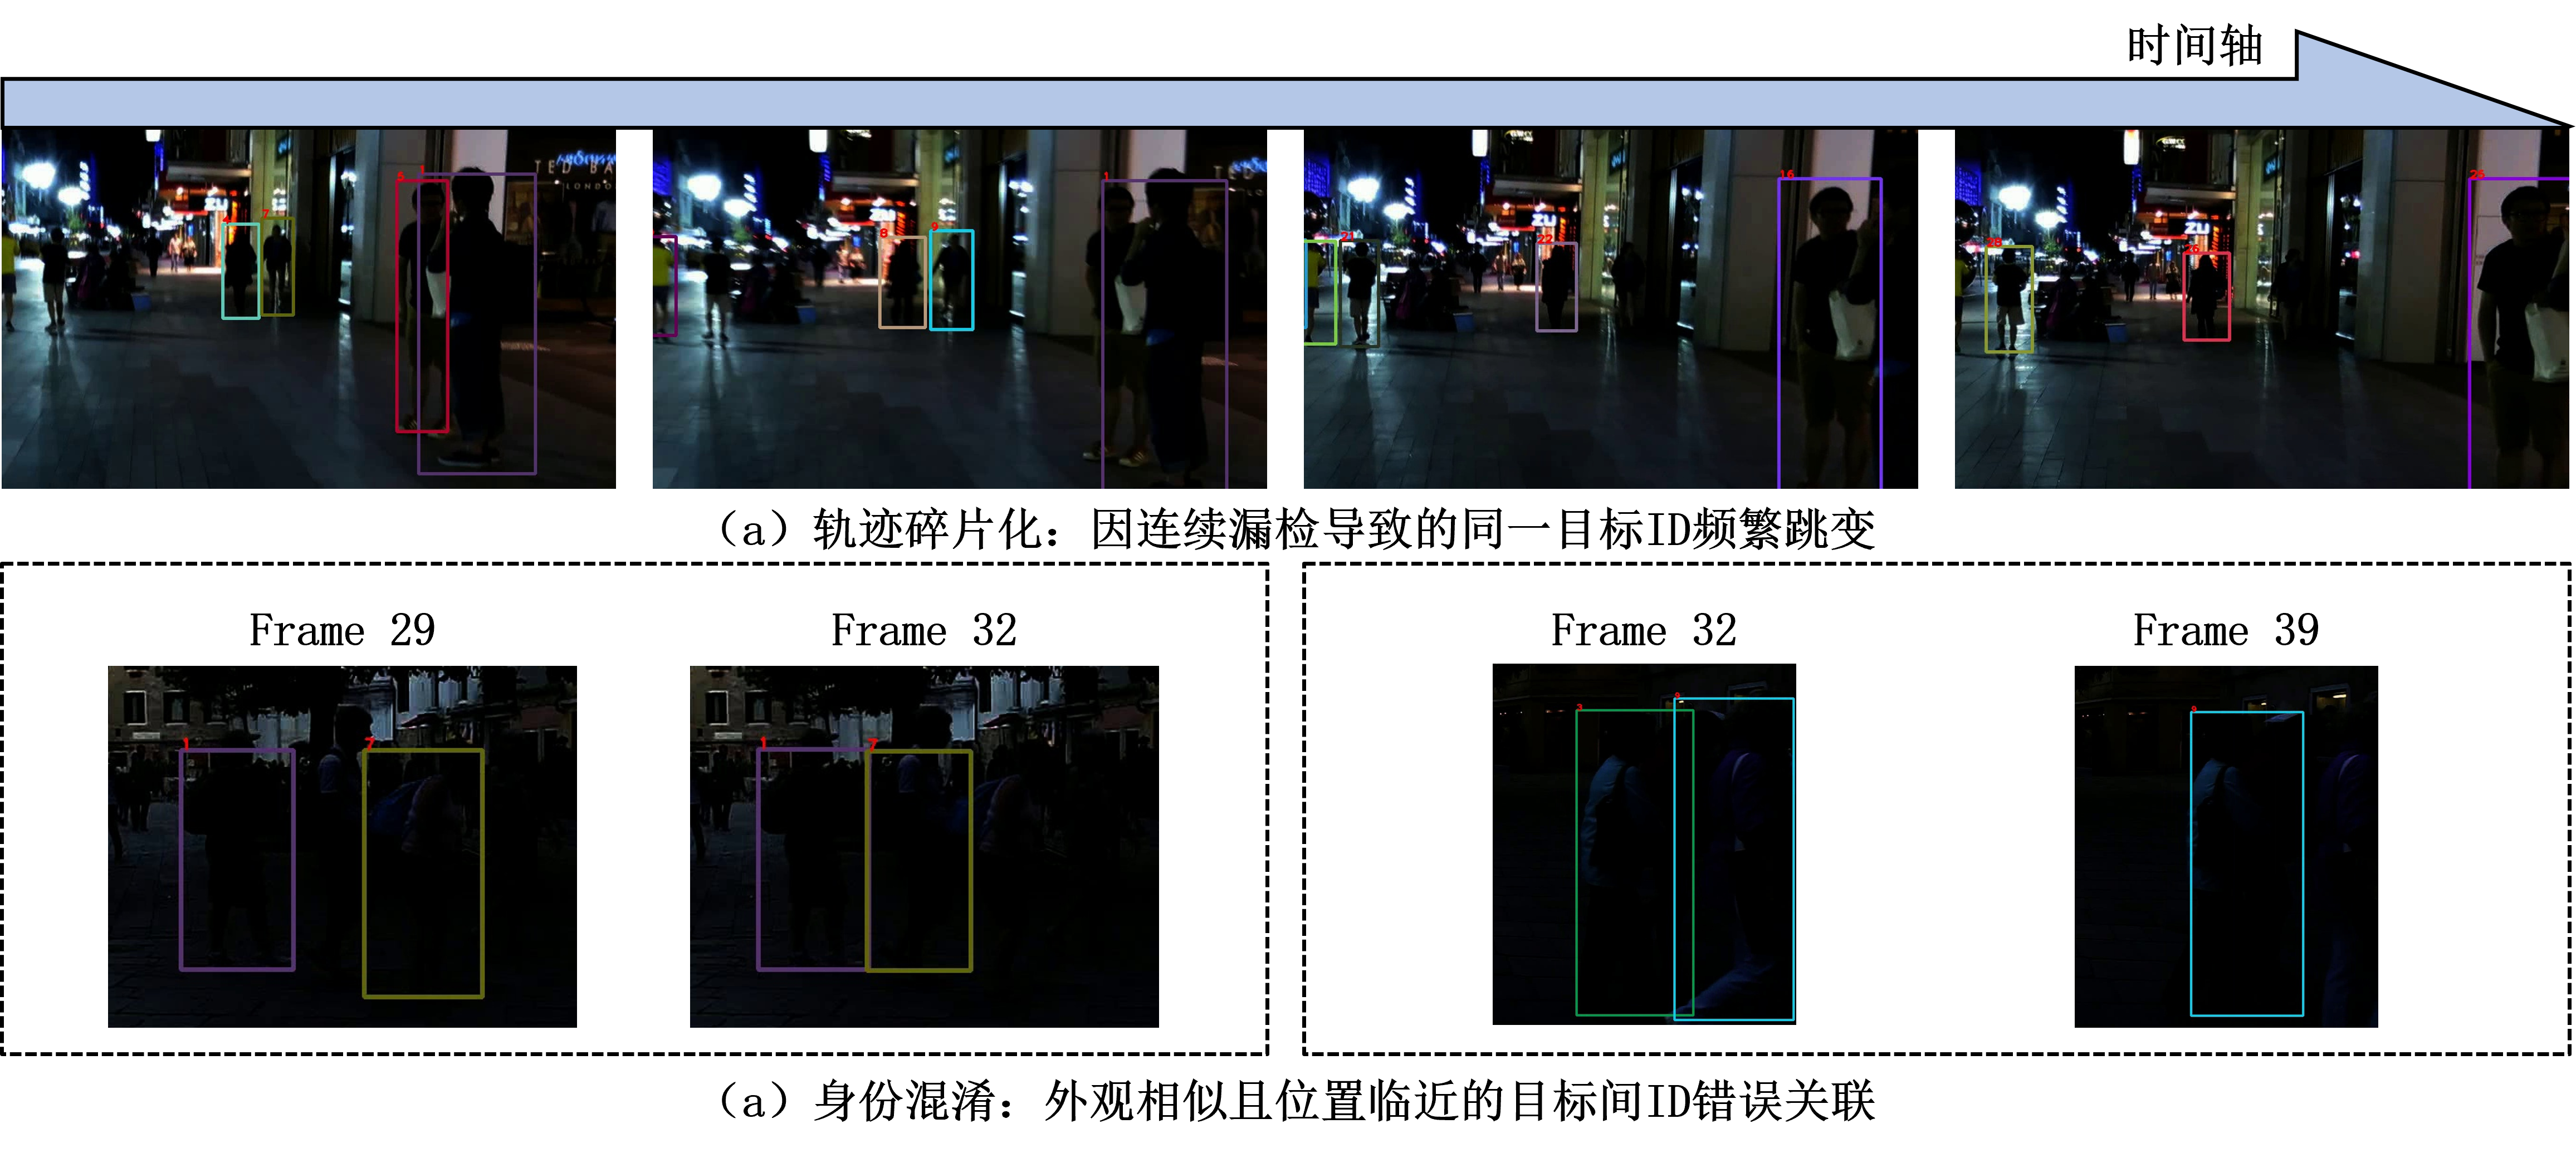
\includegraphics[width=15cm]{chapter2/2.png}
    \caption{\label{fig:ch2_2}域偏移对目标检测性能的影响示例}
\end{figure}

\subsection{域适应与领域偏移的理论定义}

在统计学习理论中,一个域(Domain)通常由特征空间 $\mathcal{X}$ 及其上的概率分布 $P(X)$ 所共同决定,
即 $\mathcal{D} = \{\mathcal{X}, P(X)\}$。
在跨域学习问题中,通常假设存在一个源域(Source Domain)
$\mathcal{D}_s = \{\mathcal{X}_s, P_s(X)\}$和一个目标域(Target Domain)$\mathcal{D}_t = \{\mathcal{X}_t, P_t(X)\}$,
且二者一般有相同或相似的任务空间,例如目标检测中的标签空间 $\mathcal{Y}$ 及其条件分布 $P(Y|X)$。

当源域与目标域之间的数据分布不一致,即$P_s(X,Y) \neq P_t(X,Y)$时,便产生了领域偏移问题。在本文研究的跨域多目标跟踪场景下,这种偏移主要表现为协变量偏移(Covariate Shift)。其数学性质满足以下两个条件:

\begin{enumerate}
    \item \textbf{边缘分布不一致}:$P_s(X) \neq P_t(X)$。这是由光照变化、大气散射(雾霾)或传感器噪声等物理因素引起的。例如,雾天图像的像素直方图分布与晴天图像存在显著差异,导致特征提取器无法正确提取有效特征。
    \item \textbf{条件分布保持一致}:$P_s(Y|X) = P_t(Y|X)$。即输入特征 $X$ 与标签 $Y$ 之间的语义映射关系保持不变。无论是在晴天还是雾天,目标的物理结构(如车辆的轮廓、行人的体态)及其所属类别的定义并未发生改变。
\end{enumerate}

因此,本文所关注的跨域自适应问题,本质上是在保证条件概率分布 $P(Y|X)$ 稳定的前提下,寻找一种有效的变换或增强策略,以此缓解源域与目标域在边缘概率分布 $P(X)$ 上的差异。

为量化与克服上述分布差异,Ben-David等人提出了著名的域适应理论\cite{ben2010theory}。该理论指出,对于假设空间 $\mathcal{H}$ 中的任意假设 $h$(即模型),其在目标域上的期望误差 $\epsilon_t(h)$ 被源域上的期望误差 $\epsilon_s(h)$ 以及两域之间的分布差异所界定:

\begin{equation}
    \label{equ:domain_bound}
    \epsilon_t(h) \leq \epsilon_s(h) + \frac{1}{2} d_{\mathcal{H}\Delta\mathcal{H}}(\mathcal{D}_s, \mathcal{D}_t) + \lambda
\end{equation}
其中,$d_{\mathcal{H}\Delta\mathcal{H}}(\mathcal{D}_s, \mathcal{D}_t)$ 表示源域与目标域在特征空间中的分布距离(Divergence),$\lambda$ 为理想联合误差常数。

由公式 \ref{equ:domain_bound} 可知,在源域误差 $\epsilon_s(h)$ 已经较低的前提下,跨域性能退化的主要来源在于源域与目标域之间的分布差异项$d_{\mathcal{H}\Delta\mathcal{H}}(\mathcal{D}_s, \mathcal{D}_t)$。
回顾\ref{subsec:cross_domain}节所述的跨域自适应方法,现有研究可进一步归纳为对$d_{\mathcal{H}\Delta\mathcal{H}}$项的两个不同层级的优化:
\begin{enumerate}
    \item \textbf{特征空间对齐}:这类方法的核心是在高维特征空间中进行操作。通过学习一个特征提取器 $\phi$,使得变换后的特征分布 $P_s(\phi(X_s))$ 与 $P_t(\phi(X_t))$ 尽可能对齐,从而直接在特征层面最小化 $d_{\mathcal{H}\Delta\mathcal{H}}$。
    \item \textbf{像素空间增强}:这类方法的核心是在原始输入空间中进行操作。它旨在学习一个增强或变换函数 $\mathcal{G}: \mathcal{X}_t \rightarrow \mathcal{X}'$,使得增强后的目标域图像分布 $P_t(\mathcal{X}')$ 能够逼近源域的清晰图像分布 $P_s(\mathcal{X}_s)$,从数据源头直接削减域偏移。
\end{enumerate}

那么,针对由雾、低光等恶劣环境引起的低级视觉退化,本文认为像素空间增强范式更具优势。
不同于在抽象的高维特征空间中进行难以解释的分布对齐,该范式能够直接针对明确的物理退化模型进行逆向校正。
这种策略不仅更直接、高效,且能更好地保持图像内容的语义一致性,为后续的检测与跟踪任务提供更可靠的输入特征。

\subsection{恶劣环境下的物理退化机制}

在本文所关注的跨域跟踪场景中,雾(Fog)与弱光(Dark)是两种典型且具有明确物理模型的退化类型。本小节旨在阐明这两种退化现象的物理机制,为后续设计数据驱动的增强模型提供理论先验。

\textbf{1. 雾天退化的大气散射模型}

雾天天气下的图像退化主要源于大气中悬浮颗粒对光的散射作用。这一过程可由经典的大气散射模型(Atmospheric Scattering Model)\cite{scatteringmodel}描述。该模型指出,传感器接收到的雾图 $I_{foggy}(x)$ 是两部分光线的叠加:
\begin{equation}
    I_{foggy}(x) = J(x)t(x) + A(1 - t(x))
    \label{equ:haze_model}
\end{equation}
其中,$I_{foggy}(x)$ 为观测到的雾天图像,
$J(x)$ 为无雾条件下的真实场景辐射图像,$A$ 为全局大气光值。
$t(x)=\exp(-\beta d(x))$ 为透射率,反映光在传播过程中未被散射的比例,
$\beta$ 和 $d(x)$ 分别表示大气散射系数与场景深度。

该模型清晰地分离了退化因素:等式右边第一项 $J(x)t(x)$ 代表直接衰减,即场景反射光在传输过程中因散射而衰减;第二项 $A(1-t(x))$ 代表大气光,即环境光被悬浮颗粒散射后进入观测路径的光线。
雾浓度越高($\beta$ 越大)或场景越远($d(x)$ 越大),透射率 $t(x)$ 越小,图像受大气光成分影响越大,导致对比度下降、颜色发白(如图\ref{fig:ch2_2}(b)所示)。
从域适应的视角看,雾的引入系统性改变了清晰图像 $J$ 的像素值分布 $P(J)$,形成了雾图分布 $P(I_{foggy})$。

\textbf{2. 低光退化的成像亮度模型}

低光照条件下的图像退化主要由环境光照不足和相机成像过程中的噪声共同导致。
其成像过程可基于Retinex理论\cite{retinex}简化建模:
\begin{equation}
    I_{dark}(x) = f\big(J(x)\big) + n(x)
    \label{equ:lowlight_model}
\end{equation}
其中,$f(\cdot)$ 表示非线性亮度映射函数(如 Gamma 压缩),
$n(x)$ 为与亮度相关的噪声项。

因此,低光退化的核心在于光照分量 $L(x)$ 的严重衰减和信噪比的急剧下降。增强的目标即是估计光照图 $L(x)$ 并抑制噪声 $N(x)$,
以恢复出在正常光照下应呈现的反射率 $R(x)$。这一过程同样是将分布 $P(I_{dark})$ 向清晰图像分布 $P(R)$ 映射的过程。

对于目标检测与跟踪任务而言,
上述两种退化机制都会直接削弱目标的可见结构信息,导致检测框定位不准、目标外观特征不稳定,
进而在时序关联过程中引发身份切换和轨迹中断问题。

\subsection{基于经典滤波器的可微图像处理器}
\label{subsec:ch2_2_3}
针对物理模型求解的病态性与计算复杂度问题,以IA-YOLO \cite{ia} 为代表的研究工作提出了一种基于可微分图像处理(Differentiable Image Processing, DIP)的自适应检测框架。
该类方法的核心思想是将传统图像信号处理(Image Signal Processor,ISP)流程中的经典滤波器进行参数化封装,使其能够作为可微分模块嵌入到深度神经网络中 \cite{erup}。
具体而言,该框架利用卷积神经网络构建参数预测器,根据输入图像的全局内容自适应地预测滤波器的关键超参数(如伽马值、锐化程度等),从而实现端到端的图像增强 \cite{gdip}。
根据处理方式与感受野的不同,这些经典滤波器通常被划分为像素级滤波器(Pixel-wise Filters)和局部滤波算子(Local Filtering Operators) \cite{erup}。

\textbf{1. 像素级滤波器}

像素级滤波器旨在对图像中的每个像素独立进行强度映射,主要用于调整图像的亮度、色彩平衡及对比度。其数学本质是定义一个从输入强度到输出强度的单调映射函数,输出值仅取决于当前像素的输入值。
假设输入像素强度为 $P_{i}=(r_{i},g_{i},b_{i})$,输出为 $P_{o}=(r_{o},g_{o},b_{o})$,常见的可微分实现形式如下:

\begin{itemize}
    \item \textbf{伽马校正(Gamma Correction)}:主要用于调整图像的整体亮度与动态范围。其数学形式为幂函数映射 $P_{o}=P_{i}^{\gamma}$。
    其中 $\gamma$ 为可学习参数:当 $\gamma < 1$ 时,图像暗部细节被提亮,适用于低光照场景;当 $\gamma > 1$ 时,图像整体变暗,适用于过曝光场景。
    
    \item \textbf{白平衡(White Balance)}:旨在消除光源色温对图像色彩的影响,恢复物体的真实颜色。它通过对RGB三个通道分别乘以增益系数 $(W_{r},W_{g},W_{b})$ 来实现,
    即 $P_{o}=(W_{r}r_{i},W_{g}g_{i},W_{b}b_{i})$。
    
    \item \textbf{对比度增强(Contrast Enhancement)}:旨在提升图像的视觉感知清晰度。通常采用S型曲线函数对图像亮度进行拉伸,压暗暗部并提亮亮部。
    例如,IA-YOLO 定义了一个可学习参数 $\alpha$ 来插值原始图像与增强图像,其公式涉及利用余弦函数构建的S曲线,用于提升感知对比度。
    公式可表示为 $P_{o}=\alpha \cdot En(P_{i})+(1-\alpha)\cdot P_{i}$,其中 $En(P_{i})$ 为基于亮度的非线性增强函数。
    
    \item \textbf{色调映射(Tone Mapping)}:主要用于高动态范围图像的压缩与调整。为了使其在神经网络中可微分,
    通常采用分段线性函数(Piecewise Linear Function)来模拟单调映射曲线。
    该方法将像素值范围 $[0, 1]$ 划分为 $L$ 个区间,每个区间具有独立的可学习斜率参数 $t_k$,从而实现对不同亮度区域的精细调整。
\end{itemize}

\autoref{fig:ch2_3}直观展示上述像素级滤波器对图像外观的影响。
\begin{figure}[htbp]
    \centering
    \includegraphics[width=15cm]{chapter2/3.png}
    \caption{\label{fig:ch2_3}典型像素级可微滤波器的增强效果示例}
\end{figure}

\textbf{2. 局部滤波算子}

与像素级滤波器不同,局部滤波算子的输出还依赖于像素的空间邻域信息,
主要用于增强图像的结构细节、抑制噪声或缓解雾霾等退化现象。

\begin{itemize}
    \item \textbf{锐化滤波器(Sharpen Filter)}:基于非锐化掩模(Unsharp Masking)原理,通过增强图像的高频分量来突出边缘与纹理。
    其可微分形式通常表示为原图与高斯模糊(Gaussian Blur)图像差分的线性组合:
    \begin{equation}
        F(x,\lambda) = I(x) + \lambda(I(x) - Gau(I(x)))
    \end{equation}
    其中 $Gau(\cdot)$ 表示高斯模糊操作,$\lambda$ 为控制锐化强度的可学习参数。当 $\lambda > 0$ 时,图像边缘被增强;当 $\lambda < 0$ 时,图像呈现平滑效果。
    
    \item \textbf{去雾滤波器(Defog Filter)}:基于暗通道先验\cite{dehaze}和大气散射模型设计。
    可微分去雾模块通常利用卷积网络估计透射率图 $t(x)$ 和全局大气光 $A$,并构建逆向复原公式:
    \begin{equation}
        J(x) = \frac{I(x) - A}{t(x)} + A
        \label{equ:defog_filter}
    \end{equation}
    通过学习透射率 $t(x)$ 的参数,网络能够自适应地去除图像中的雾霾影响,恢复场景的清晰度和对比度。
\end{itemize}

\autoref{fig:ch2_4}直观展示上述局部滤波算子对图像外观的影响。
\begin{figure}[htbp]
    \centering
    \includegraphics[width=15cm]{chapter2/4.png}
    \caption{\label{fig:ch2_4}典型局部滤波算子的增强效果示例}
\end{figure}

综上所述,基于经典设计的像素级滤波器与局部滤波算子构成了现有可微图像处理(DIP)方法的基础组件。
通过将传统图像增强算子进行参数化并嵌入深度网络,该范式在一定程度上实现了物理可解释性与端到端可优化性的统一,为跨域视觉感知任务提供了一种有效的增强路径。
然而,在实际应用中,这种基于滤波器组合的设计仍面临若干局限:一方面,不同滤波器对应的参数空间具有不连续性,增加了整体优化难度;另一方面,滤波器之间可能存在功能耦合现象(例如去雾操作引入噪声放大),且其执行顺序往往依赖人工经验进行设定,难以针对具体任务自适应调整。
因此,如何在保持经典滤波器可解释优势的同时,进一步提升增强结构的灵活性与任务适配能力,仍是跨域自适应视觉建模中亟需解决的问题。

\section{数据集与评价方法}
为保证实验评估的规范性与可比性,本节对本文实验所使用的数据集与评价指标进行说明。根据研究内容的技术侧重点,本节细分成跟踪与检测两部分:第一部分
介绍多目标跟踪任务中常用的基准数据集与评价指标;第二部分则阐述跨域检测任务相关的数据集与评价指标。
\subsection{多目标跟踪数据集与评价指标}
\label{subsec:ch2_3_1}
\textbf{1. 多目标跟踪数据集}

为验证多目标跟踪算法在复杂场景下的性能,本文主要选用公开的多目标跟踪基准数据集MOT16\cite{mot16}和MOT17\cite{mot16}上进行评估。这两个数据集由 MOT Challenge 系列竞赛组织者维护,是当前多目标跟踪领域最权威的基准数据集之一,广泛用于算法性能对比与鲁棒性测试。 

MOT16数据集是在MOT15\cite{mot15}的基础上于2016年发布的改进版本。针对之前数据集标注不统一的问题,MOT16对所有视频序列进行了重新标注,确保了标注规则的严格统一,从而消除了由标注差异带来的评估误差。
该数据集共包含14个视频序列,被均分为训练集(7个序列)和测试集(7个序列)。相比于早期的跟踪数据集,MOT16具有更高的人群密度,总计包含11,235帧视频、1,276条目标运动轨迹以及292,733个目标边界框。
在公共检测(Public Detection)方面,MOT16提供了基于DPM\cite{DPM}检测器的检测结果作为输入,以供研究人员在统一的检测基准下评估跟踪性能。

MOT17数据集则在MOT16的基础上进一步优化,保留了相同的视频序列和划分方式,但提供了更精确的标注。MOT17的总帧数与MOT16相同(11,235帧),但目标轨迹数增加至1,331条,检测框总数达到300,373个。
除DPM检测器外,MOT17还额外提供了基于Faster R-CNN\cite{FasterRCNN}和SDP\cite{SDP}检测器的检测结果,共计三组不同质量的检测数据。这一设计使得研究者能够系统分析检测器性能对跟踪算法的影响,从而更全面地评估算法的鲁棒性。

如\autoref{fig:ch2_5}所示,MOT16/17数据集涵盖了多样化的真实场景。其挑战性主要体现在以下三个方面:
\begin{figure}[htbp]
    \centering
    \includegraphics[width=15cm]{chapter2/5.png}
    \caption{\label{fig:ch2_5}MOT数据集典型场景实例}
\end{figure}

\textbf{(1) 场景与视角多样性}:包含城市街道、广场、室内走廊等多种环境,拍摄视角涵盖平视、俯视及移动视角。

\textbf{(2) 目标密度变化大}:视频帧序列中行人密度从稀疏到高度密集不等,密集场景下严重的遮挡是导致目标丢失和身份切换的主要原因。

\textbf{(3) 动态条件复杂}:包含相机静止与运动(手持、车载)的情况,且同一场景可能包含白天、夜晚或光照剧烈变化的片段,对目标的外观特征提取与运动模型预测构成极大挑战。


\textbf{2. 多目标跟踪评价指标}

多目标跟踪的任务要求算法在准确识别与定位视频帧中多个目标的同时,为其分配唯一的身份标识(Identity, ID)并建立时空轨迹。为了衡量一个跟踪系统的性能,通常要求其满足以下准则:
\begin{itemize}
    \item 检测覆盖率:算法应尽可能识别并跟踪视频序列中每一帧出现的全部真实目标;
    \item 定位精确度:所提取的目标边界框位置应尽可能贴合真实目标的实际位置,减小几何误差;
    \item 身份一致性:在目标的整个生命周期内,系统应为其分配并保持一致且唯一的编号,避免在遮挡或运动突变时发生身份频繁切换。
\end{itemize}

那么,为全面评估算法的跟踪性能,本文采用当前多目标跟踪领域中广泛使用的三类评价指标,
包括 CLEAR MOT 指标 \cite{clear}、IDF1 指标 \cite{idf1} 以及 HOTA 指标 \cite{hota}。

\textbf{(1) CLEAR指标}

CLEAR指标是多目标跟踪领域最基础的评价指标体系,其中最核心的指标是多目标跟踪准确度(Multiple Object Tracking Accuracy,MOTA)。MOTA综合考虑了误检(False Positives,FP)、漏检(False Negatives,FN)以及身份切换(Identity Switches, IDSW)三种错误类型,能够直观反映跟踪器的整体性能。
其计算公式如下:
\begin{equation}
    \text{MOTA} = 1 - \frac{\sum_{t}(FN_t + FP_t + IDSW_t)}{\sum_{t}GT_t}
    \label{equ:mota}
\end{equation}
其中,$t$表示帧序列,$GT_t$为第$t$帧中真实目标的总数。MOTA越高,代表算法在检测与初级关联方面的性能越好。

此外,多目标跟踪精确度(Multiple Object Tracking Precision,MOTP)用于衡量预测位置框与真实位置框之间的空间重叠度,计算公式为:
\begin{equation}
    \text{MOTP} = \frac{\sum_{i,t} d_{i,t}}{\sum_{t} c_t}
    \label{equ:motp}
\end{equation}
其中,$d_{i,t}$表示第$t$帧中第$i$个预测框与真实框之间的交并比(Intersection over Union,IOU),$c_t$为第$t$帧成功匹配的目标数。MOTP越高,表示算法在定位精度方面表现越佳。

\textbf{(2) IDF1指标}

为了弥补MOTA对身份一致性关注不足的问题,IDF1指标被提出用于专门衡量跟踪结果中的身份保持能力。它将跟踪问题视为身份分类问题,计算基于身份匹配的精确率和召回率的调和平均数:
\begin{equation}
\text{IDF1} = \frac{2 \cdot \text{IDTP}}{2 \cdot \text{IDTP} + \text{IDFP} + \text{IDFN}}
\end{equation}
其中,$\text{IDTP}$表示身份匹配正确的检测数(Identity True Positives),$\text{IDFP}$ 表示身份匹配错误的检测数(Identity False Positives),$\text{IDFN}$表示身份漏匹配的检测数(Identity False Negatives)。IDF1越高,表明算法在长时跟踪中保持身份ID稳定的能力越强。

\textbf{(3) HOTA指标}

HOTA(Higher Order Tracking Accuracy)是近年来提出的一种新型多目标跟踪评价指标,其核心思想是将检测性能与关联性能进行统一建模,从而对跟踪结果进行更加平衡和全面的评估。

HOTA指标定义为在不同匹配阈值下检测准确率与关联准确率的集合平均,计算公式为:
\begin{equation}
\text{HOTA} = \sqrt{\text{DetA} \cdot \text{AssA}}
\end{equation}
其中,$\text{DetA}$ 表示检测准确率(Detection Accuracy),用于衡量目标是否被正确检测;$\text{AssA}$ 表示关联准确率(Association Accuracy),用于衡量目标在时间维度上的身份一致性。

HOTA 指标能够在检测质量与关联质量之间取得良好的平衡,避免单一指标过度偏向检测或关联问题,因此逐渐成为当前多目标跟踪评测中极具代表性的综合性指标。

\subsection{跨域目标检测数据集与评价指标}
\label{subsec:ch2_3_2}
\textbf{1. 跨域目标检测数据集}

为验证本文所提出的跨域自适应增强方法在缓解视觉退化、提升模型泛化能力方面的有效性,本文选用PASCAL VOC 2007\cite{voc07}、PASCAL VOC 2012\cite{voc12}、ExDark\cite{Exdark}和RTTS\cite{rtts}四个具有代表性的数据集,涵盖从理想光照到极端退化环境的多样性需求。
\autoref{fig:ch2_6}直观展示了这四个数据集的典型样本及其对应的视觉条件。
\begin{figure}[htbp]
    \centering
    \includegraphics[width=15cm]{chapter2/6.png}
    \caption{\label{fig:ch2_6}跨域检测实验所用数据集视觉对比示例}
\end{figure}

\textbf{(1) PASCAL VOC 数据集}

PASCAL VOC 是目标检测领域中最经典、应用最广泛的通用检测数据集之一。
本文采用 VOC2007 与 VOC2012 数据集作为源域训练数据,其包含 20 个常见目标类别,如 \textit{person}、\textit{car}、\textit{bus}、\textit{train} 等,覆盖了日常交通与城市环境中的主要目标类型。

VOC2007 数据集包含 5011 张训练与验证图像以及 4952 张测试图像,VOC2012 数据集包含 11540 张训练与验证图像。该数据集采集于光照良好、成像清晰的自然场景,图像质量较高、标注规范,通常被视为理想环境下的标准检测基准。
因此,在跨域实验中,VOC数据集被用作源域数据,用于训练基础目标检测模型。

\textbf{(2) ExDark 数据集}

ExDark(Exclusively Dark dataset)是一个专门针对弱光环境构建的目标检测数据集,
旨在评估检测算法在极端低照度条件下的鲁棒性。
该数据集包含约 7363 张低光照图像,
图像来源涵盖室内、室外、夜间街景等多种真实场景,
具有显著的亮度不足、噪声干扰与颜色失真等特征。

ExDark 数据集共标注了 12 类目标,
其中包括 \textit{person}、\textit{car}、\textit{bicycle} 等与交通场景密切相关的类别。
由于其成像条件与 VOC 数据集存在明显差异,
ExDark 被广泛用于评估跨域检测与低光增强算法的有效性。
在本文中,
ExDark 作为弱光条件下的目标域数据集,
用于验证所提出自适应增强方法对低光场景检测性能的提升能力。

\textbf{(3) RTTS 数据集}

RTTS(Real-world Task-driven Testing Set)数据集是 RESIDE 去雾数据集的一部分,
专门用于真实雾天场景下的目标检测任务评估。
该数据集包含来自真实道路与城市环境的雾天图像,
具有明显的大气散射效应,
表现为图像对比度下降、颜色泛白以及远处目标模糊等特征。

RTTS 数据集为每张图像提供了目标检测标注,主要涵盖 \textit{car}、\textit{bus}、\textit{person}、\textit{bicycle} 等交通相关目标类别,
非常适合用于评估雾天条件下目标检测算法的鲁棒性。
在本文中,RTTS 数据集作为雾天场景下的目标域数据,用于验证所提出方法在去雾增强与检测协同方面的有效性。

\textbf{2. 目标检测评价指标}

为定量评估目标检测算法在不同数据集上的检测性能,本文采用目标检测领域中最常用的平均精度指标(Mean Average Precision, mAP)作为评价标准。

在给定类别$c$的情况下,其平均精度(Average Precision, AP)定义为精确率–召回率(Precision–Recall)曲线下的面积,用于综合衡量检测结果的准确性与完整性。
当预测框与真实框之间的交并比(Intersection over Union, IoU)满足:
\begin{equation}
\text{IoU} = \frac{\text{Area}(B_p \cap B_{gt})}{\text{Area}(B_p \cup B_{gt})} \geq \tau
\end{equation}
则该预测被视为正确检测,其中$B_p$和$B_{gt}$分别表示预测边界框与真实边界框,$\tau$为IoU阈值。

本文主要采用$\tau = 0.5$的设置,即常用的$\text{mAP@0.5}$指标,并对所有类别的$\text{AP}$取平均,其定义为:
\begin{equation}
\text{mAP} = \frac{1}{C} \sum_{c=1}^{C} \text{AP}_c
\end{equation}
其中 $C$ 表示目标类别总数。

mAP 指标能够直观反映检测算法在不同类别上的综合检测性能,
在跨域检测实验中,通过对比源域与目标域上的 mAP 变化,可以有效衡量域偏移对检测性能的影响,以及自适应增强方法在缓解跨域性能退化方面的作用。
\section{本章小结}
本章系统阐述了支撑本文后续研究的核心理论基础与实验评估框架。首先,深入介绍了图神经网络的基本概念、谱域与空域方法体系,重点剖析了基于消息传递的空域建模范式,
为第三章提出的基于图神经网络的轨迹关联方法奠定了坚实的理论基础。
其次,从域适应理论出发,分析了跨域视觉感知中的分布偏移问题,
阐明了雾天与低光环境的物理退化机制,并系统梳理了可微分图像处理的前沿方法,为第四章设计跨域自适应增强算法提供了清晰的理论指引和技术依据。
最后,对本文实验所采用的多目标跟踪与跨域检测数据集及评价指标进行了说明,为第三章和第四章的算法验证与实验分析奠定了统一且规范的评测基础。